%-------------------------------------------------------------------------------
%                            BAB IV
%               		HASIL DAN PEMBAHASAN
%-------------------------------------------------------------------------------

\chapter{HASIL DAN PEMBAHASAN}
	\section{Analisis Kebutuhan Sistem}
		Bagian ini menjelaskan hal-hal yang terkait tentang pengembangan aplikasi sebelum penulisan code sesumber.

		\subsection{Fitur-Fitur Aplikasi}
			Kemampuan menangani sensor-sensor:
			\begin{itemize}
				\item Mampu membaca dan menampilkan suhu yang terbaca pada sensor IQRF,
				\item mampu menyala-matikan relay pada peranti yang diinginkan,
				\item mampu menambah dan mengurangi peranti baru baik IQRF atau XBee,
				\item mampu menjalankan profile tertentu dari kombinasi suhu dan relay atau waktu tertentu.
			\end{itemize}

			Kemampuan menangani pengguna:
			\begin{itemize}
				\item Mengharuskan pengguna untuk memasukkan nama dan kata sandi sebelum masuk ke aplikasi,
				\item dapat menambah atau mengurangi pengguna yang dapat memasuki sistem.
			\end{itemize}

		\subsection{\emph{Use Case Diagram}}
			\begin{figure}[ht!]
			  \centering
			    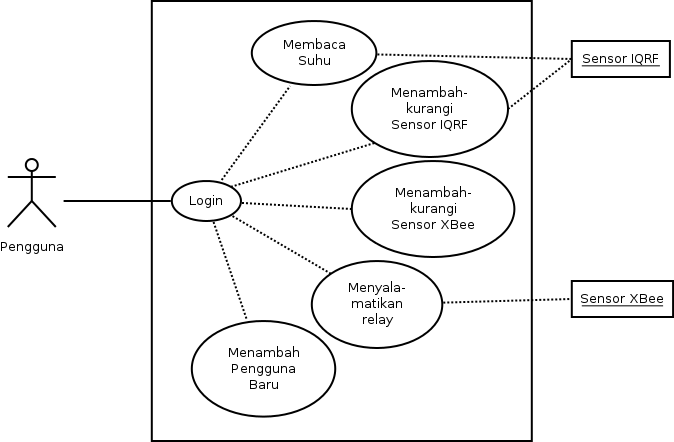
\includegraphics{gambar/usecase}
			    \caption{Diagram \emph{use case} dari penelitian.}
			    \label{usecase}
			\end{figure}

		\subsection{Diagram Arsitektur Sistem}
			\begin{figure}[ht!]
			  \centering
			    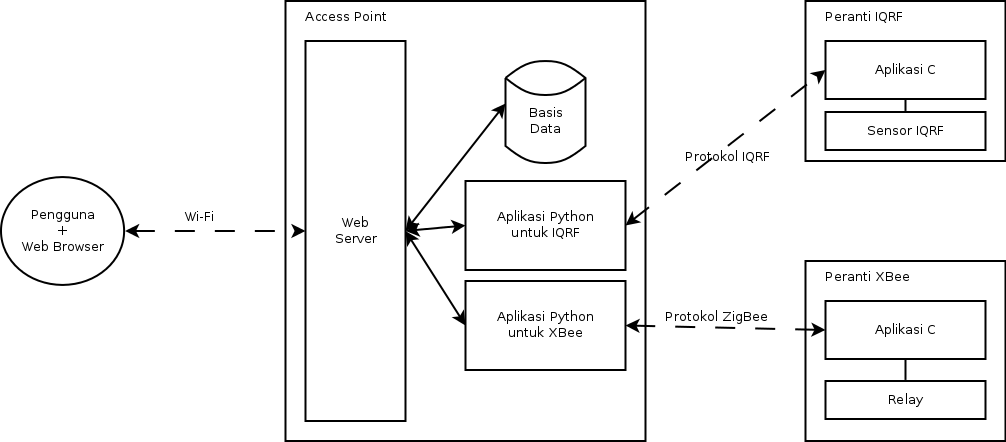
\includegraphics{gambar/system-architecture}
			    \caption{Diagram Arsitektur Sistem.}
			    \label{system-architecture}
			\end{figure}

		\subsection{SDLC}
			\begin{figure}[ht!]
			  \centering
			    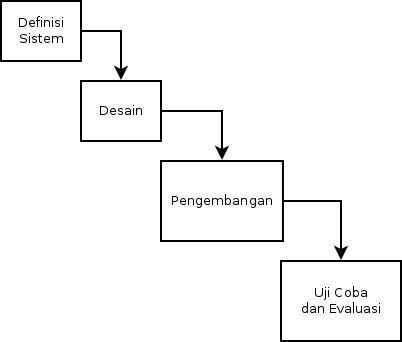
\includegraphics{gambar/sdlc}
			    \caption{Diagram SDLC.}
			    \label{sdlc}
			\end{figure}
	
	\section{Perancangan Aplikasi}
		Bagian ini menjelaskan hal-hal terkait pengembangan aplikasi.

		\subsection{Peta Situs}
			\begin{figure}[ht!]
			  \centering
			    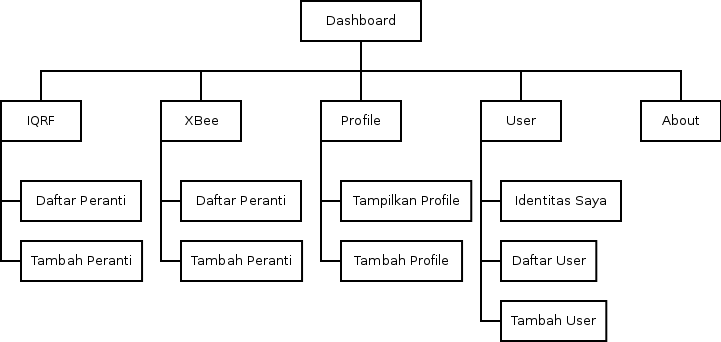
\includegraphics{gambar/sitemap}
			    \caption{Peta situs aplikasi web.}
			    \label{sitemap}
			\end{figure}

		\subsection{Diagram Alir Proses}
			Diagram alir menambah peranti IQRF:

			\begin{figure}[ht!]
			  \centering
			    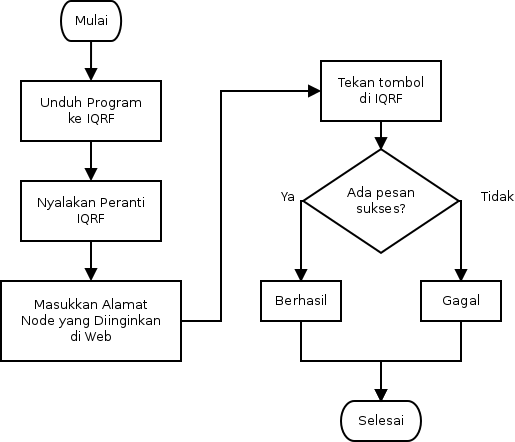
\includegraphics{gambar/add-iqrf}
			    \caption{Diagram Alir Penambahan Peranti IQRF ke Aplikasi.}
			    \label{add-iqrf}
			\end{figure}

			Diagram alir menambah peranti XBee:

			\begin{figure}[ht!]
			  \centering
			    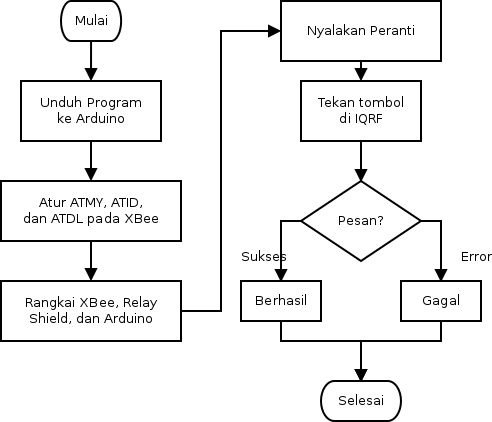
\includegraphics{gambar/add-xbee}
			    \caption{Diagram Alir Penambahan Peranti XBee ke Aplikasi.}
			    \label{add-xbee}
			\end{figure}

		\subsection{Persiapan Pra Pengembangan Aplikasi}
			\begin{enumerate}
				\item Konfigurasi Router/AP

					Penelitian ini menggunakan AP keluaran TP-LINK seri MR3020. AP jenis ini dipilih karena bentuknya yang kecil sehingga mudah dibawa atau dipindahkan dan kemudahannya untuk dimodifikasi. TP-LINK MR3020 juga terbilang populer di ranah komunitas sistem benam (\emph{embedded device}) sehingga memiliki dukungan yang baik dari pabrikan dan komunitas. 

					Sebelum digunakan, \emph{firmware} bawaan TP-LINK MR3020 harus diganti dengan sistem operasi OpenWRT. Proses penggantian cukup mudah karena hanya memanfaatkan menu \emph{firmware upgrade} dari web admin yang sudah tersedia.	Sistem Operasi OpenWRT yang digunakan adalah Attitude Adjustment versi 12.09 dengan Linux kernel 3.3.8. \emph{Image file} sistem operasi tersebut bisa diunduh secara gratis pada situs \url{www.openwrt.org}.

					Setelah OpenWRT berhasil terinstall, langkah selanjutnya adalah mengimplementasikan \emph{extroot}. \emph{Extroot} dapat memperbesar memori penyimpanan dengan bantuan USB \emph{flash drive}. Langkah yang harus dilakukan pertamakali adalah menginstall perangkat lunak dengan perintah sebagai berikut:
					\begingroup
					    \fontsize{10pt}{12pt}\selectfont
					    \begin{verbatim}
							opkg update
							opkg install block-extroot block-hotplug block-mount
					    \end{verbatim}  
					\endgroup

					Kemudian dilanjutkan dengan menyalin isi dari memori internal TP-LINK MR3020 ke USB \emph{flash drive} yang di-\emph{mount} pada direktori /mnt/sda1 dengan perintah:
					\begingroup
					    \fontsize{10pt}{12pt}\selectfont
					    \begin{verbatim}
							tar -C /overlay -cvf - . | tar -C /mnt/sda1 -xf -
					    \end{verbatim}  
					\endgroup

					Langkah terakhir adalah mengkonfigurasi file /etc/config/fstab dan menyalakan ulang AP. Konfigurasi diganti dengan detil sebagai berikut:
					\begingroup
					    \fontsize{10pt}{12pt}\selectfont
					    \begin{verbatim}
							config mount
						        option target        /mnt
						        option device        /dev/sda1
						        option fstype        ext3
						        option options       rw,sync
						        option enabled       1
						        option enabled_fsck  0
						        option is_rootfs     1
					    \end{verbatim}  
					\endgroup

				\item Konfigurasi Komputer untuk Pengembangan
			\end{enumerate}
		\subsection{Pengembangan Aplikasi WSN}
		\subsection{Pengembangan Aplikasi Python}
		\subsection{Pengembangan Aplikasi Berbasis Web}
		\subsection{Evaluasi dan Perbaikan}
		\subsection{\emph{Screenshot} Aplikasi}
		\subsection{Kode Sesumber}
			Kode sesumber dapat diperoleh pada situs GitHub dengan alamat URL \url{https://github.com/gtrdp/wsn-ip-interoperability}.


	\section{Analisis Unjuk Kerja Aplikasi}
		Bagian ini menjelaskan hal-hal terkait instalasi aplikasi ke kondisi sesungguhnya, hasil uji coba, masalah, dan penyelesaian.

		\subsection{Hasil Akhir Perangkat Keras}
		\subsection{Instalasi Aplikasi}
		\subsection{Hasil Uji Coba Aplikasi}
		\subsection{Masalah dan Penyelesaian}
